%!TEX root = ../thesis.tex
%*******************************************************************************
%****************************** Third Chapter **********************************
%*******************************************************************************
\chapter{Design}
\graphicspath{{Chapter5/Figs/Raster/}{Chapter5/Figs/}}

Following the discussion in Chapter 2.3.1 and 2.5, the designs for this project 
will be created on top of Hyperledger Fabric, a public permissioned blockchain.
It has become clear that a blockchain specific, high-fidelity prototyping tool is needed 
to create system designs such as data and transaction models.

\section{Design Tool}

Hyperledger Composer is an open source development toolset and framework that aims to 
accelerate time to value for blockchain projects. It offers business-centric 
abstractions, allowing business owners and developers to rapidly develop 
use cases and model a blockchain network. The design tools offered take the forms of:
\begin{itemize}
    \setlength\itemsep{0em}            
    \item An object-oriented modelling language (.cto file) to define data models in 
    the blockchain network for assets, participants and transactions
    \item JavaScript functions (.js file) to define logic for smart contracts triggered by transactions
    \item An access control language (.acl file) to define access rules for records on the blockchain\\
    \citep{official2018composer}
\end{itemize}

See Figure \ref{fig:composer2fabric} for a visual explainer of how Hyperledger Composer 
helps designers and developers create these high level definitions.

\begin{figure}[!ht] 
    \centering    
    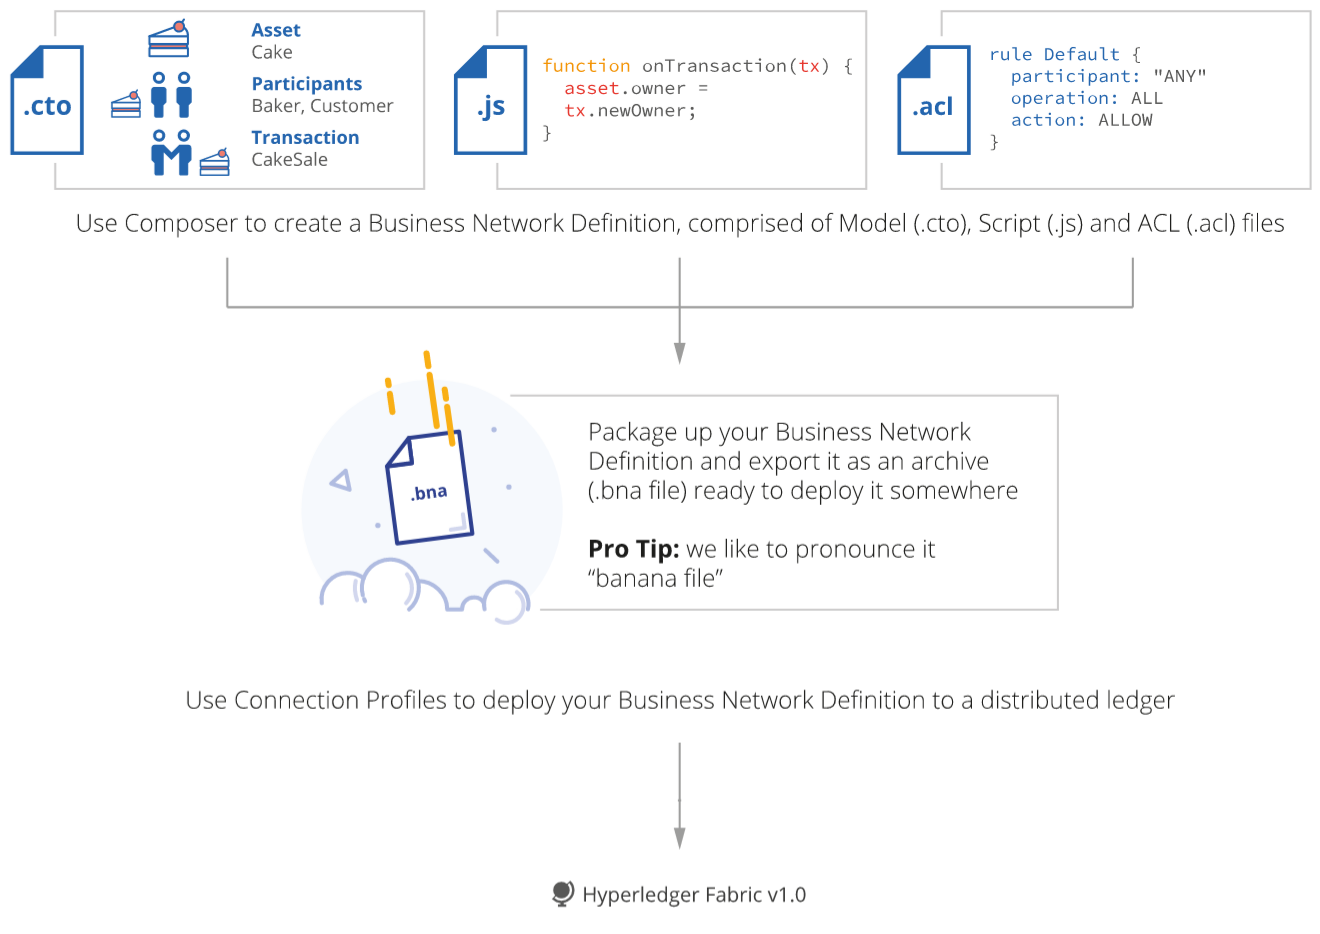
\includegraphics[width=1.0\textwidth]{composer2fabric}
    \caption[Hyperledger Composer]
        {Components in the Hyperledger Composer framework and how it deploys to 
        Hyperledger Fabric \citep{cuicapuza2017composer}} 
    \label{fig:composer2fabric}
\end{figure}
% https://medium.com/@RichardCuica/hyperledgers-fabric-composer-simplifying-business-networks-on-blockchain-94313b979671

A significant advantage of using Hyperledger Composer is its ability to package these 
prototype definitions and deploy it to Hyperledger Fabric, our target blockchain platform. 
This will speed up the implementation of the proposed demonstrator applications 
in the next stage.

Throughout the design process, the Hyperledger Composer notations are converted into UML sequence 
diagrams, class diagrams and activity diagrams with PlantUML, an open source language-to-diagram drawing tool.

The discussion below may regularly refer back to the functional requirements (FR) and 
non-functional requirements (NR) defined in the previous Chapter 4.

\section{Transaction Sequences}

A transaction is the only activity that a peer can perform to alter the state of the blockchain. 
Designing the sequences of transactions necessary to fulfil the desired use journeys will  
be able to provide a good overview of the work ahead, and the fields that data model 
objects should include to enable these transactions. Two overarching use cases are considered: 
assessment and curriculum personalisation.

\subsection{Assessment}

These four transactions are required to complete the assessment use case:
\begin{itemize}
    \setlength\itemsep{0em}        
    \item CreateModule: a transaction ordered by a teacher to store metadata about a course module, 
    its units and assessments onto the blockchain;
    \item AddSubmission: a transaction ordered by a learner to store a submission (assessment attempt) 
    on the blockchain, this could return the result of the assessment if the result is returned by 
    an automatic (machine) marking service;
    \item SubmitResult: a transaction ordered by a teacher to store details of an assessor assessment 
    on the blockchain;
    \item GenCertificate: a transaction ordered by a teacher to create a new certificate on the blockchain.
\end{itemize}

See Figure \ref{fig:assessmentloop} for where these transactions occur in a sequence diagram.

\begin{figure}[!ht] 
    \centering    
    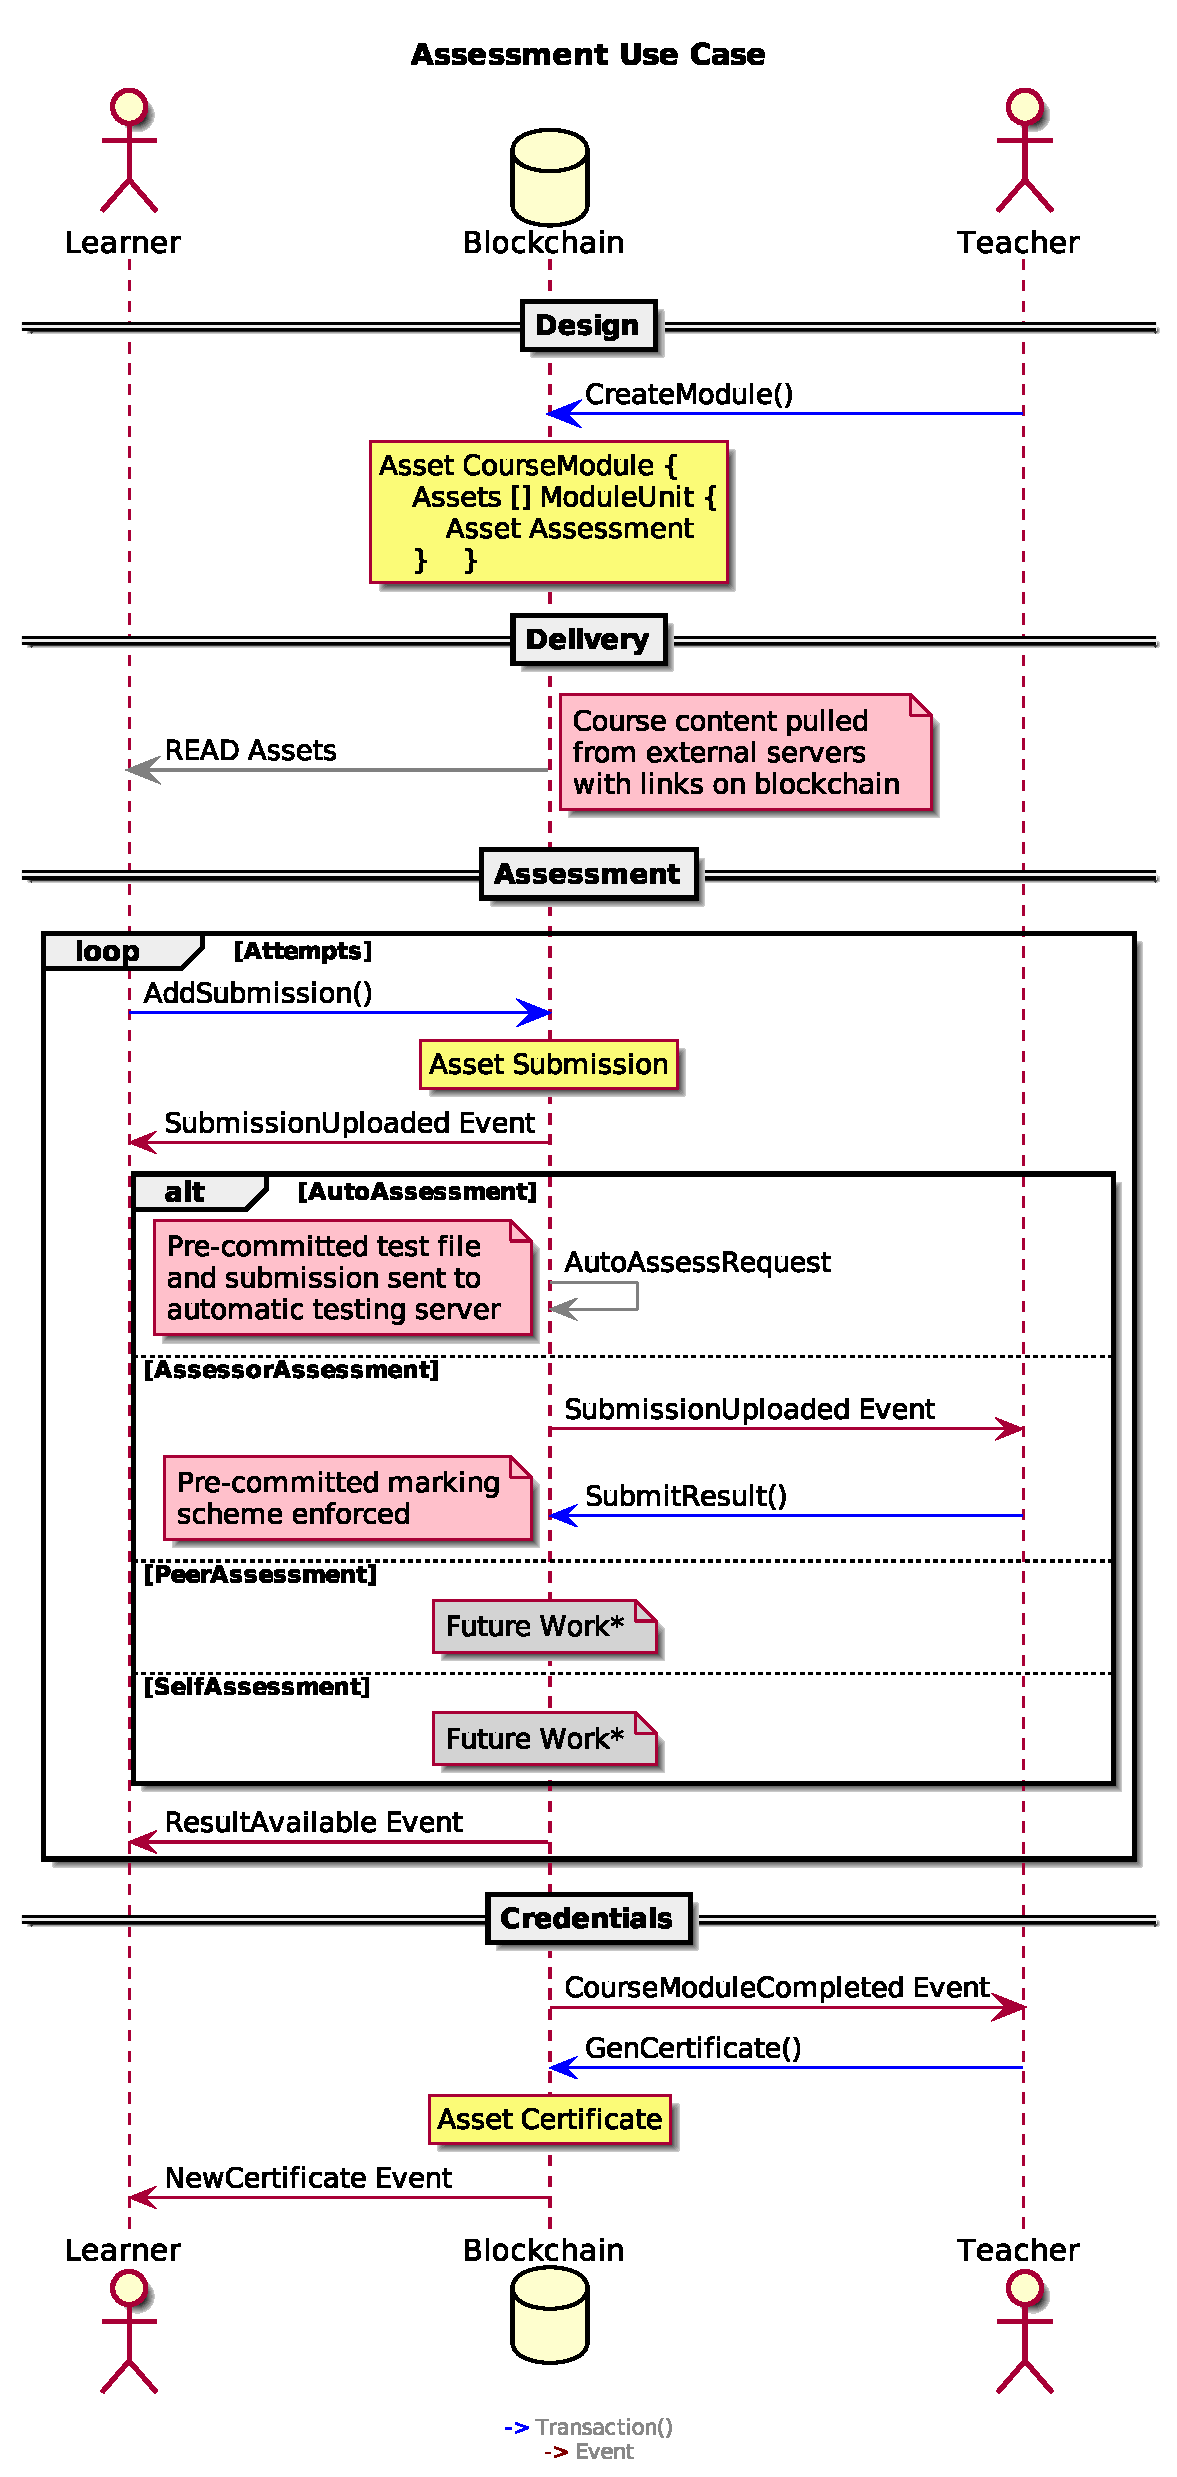
\includegraphics[width=0.65\textwidth]{assessmentloop}
    \caption[Assessment Use Case]
        {A UML sequence diagram denoting the assets, transactions and events between 
        learner and teacher participants on the blockchain for the assessment use case} 
    \label{fig:assessmentloop}
\end{figure}

\subsection{Curriculum Personalisation}

Similarly, we looked at the transactions required to build a minimum viable product 
that facilitates curriculum personalisation. A curriculum here is simply a list of course 
modules attached to a learner and a teacher (a personal tutor for the learner).

\begin{itemize}
    \item ProposeCurriculum: a transaction ordered by a learner or a teacher to propose 
    a brand new curriculum, or to proposed edits to an existing curriculum on the blockchain.
    \item ApproveCurriculum: a transaction ordered by a teacher to enrol a learner to 
    the course modules in the learner's curriculum.
\end{itemize}

See Figure \ref{fig:personalisationloop} for where these two transactions occur in a sequence diagram.

\begin{figure}[!ht] 
    \centering    
    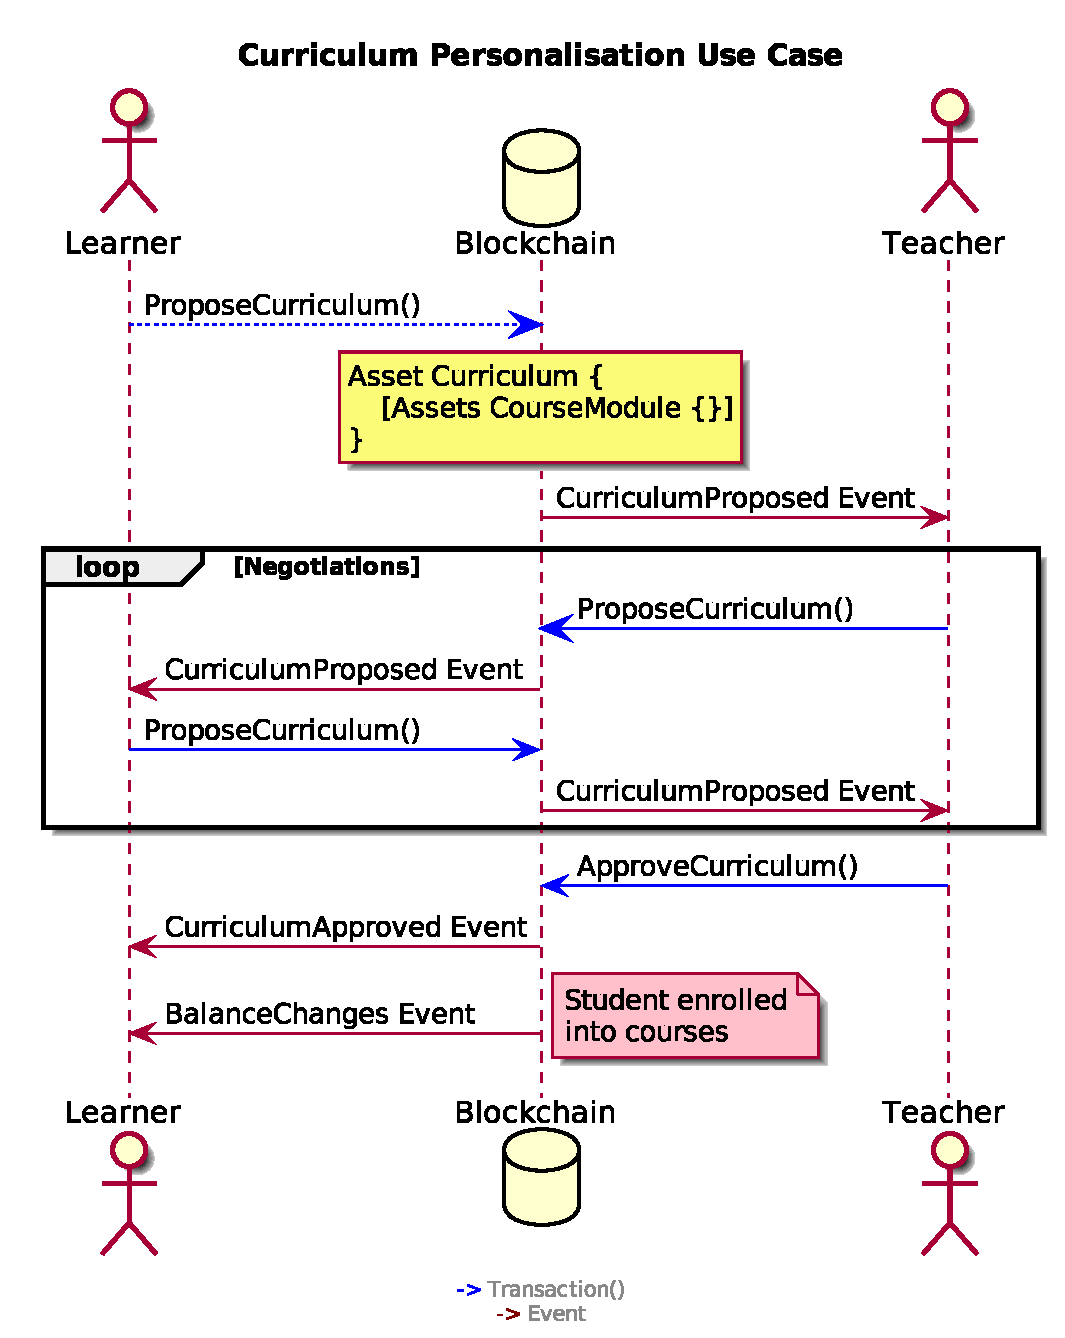
\includegraphics[width=0.7\textwidth]{personalisationloop}
    \caption[Curriculum Personalisation Use Case]
        {Sequence diagram denoting the assets, transactions and events between 
         learner and teacher participants on the blockchain for the curriculum personalisation use case} 
    \label{fig:personalisationloop}
\end{figure}

% automatic formative assessments Annette's student

% schema --> reviewer

\section{Participant, Asset and Transaction Models}

\subsection{Participants}

The network definitions will involve three main types of participants: 
\begin{itemize}
    \setlength\itemsep{0em}    
    \item teachers (which can be lecturers, teaching assistants, tutors, etc.)
    \item learners (which can be campus students, distant learners, etc.)
    \item readers (members of the public who are interested in querying or verifying records, 
    such as employers and further education providers)
\end{itemize}

See Figure \ref{fig:participants} for the detailed entity properties of these three participant types 
in a class diagram.

\begin{figure}[!ht] 
    \centering    
    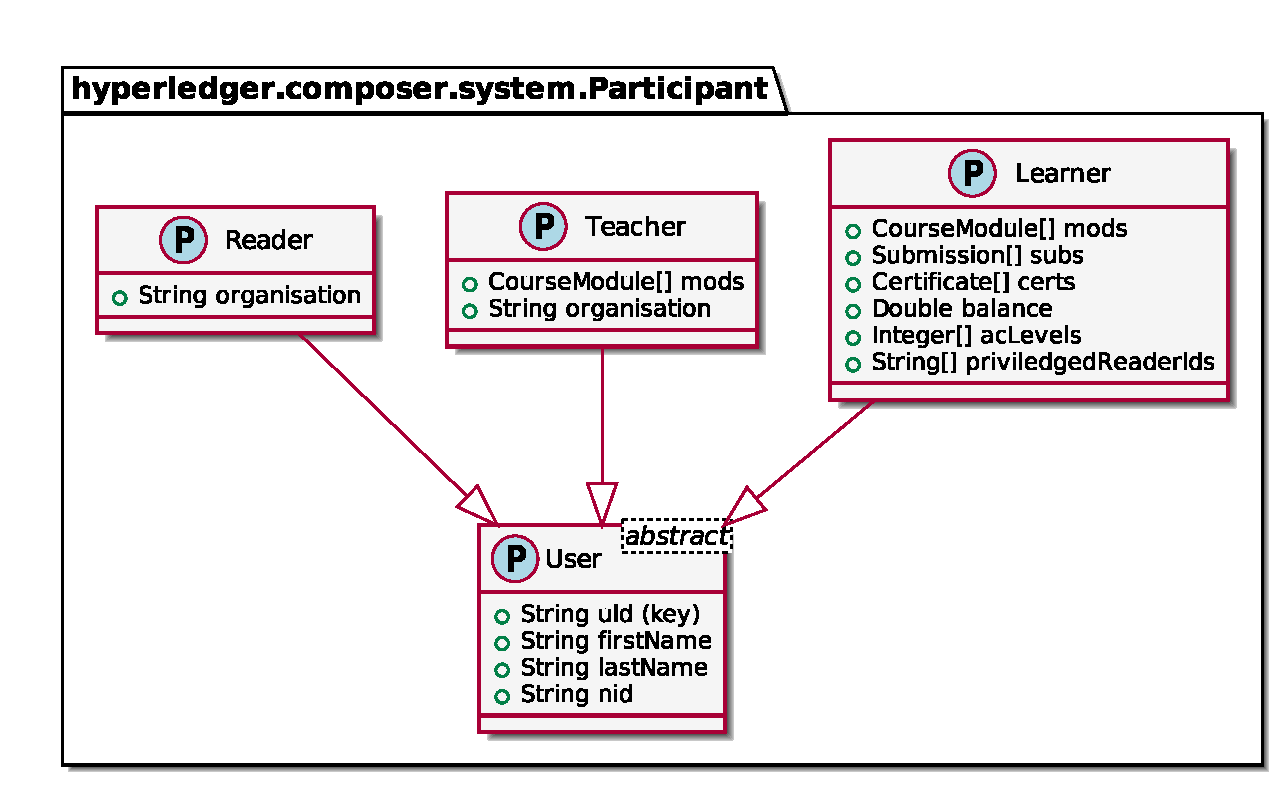
\includegraphics[width=0.7\textwidth]{participants}
    \caption[Participants Class Diagram]
        {A UML class diagram describing the learner, teacher and reader participants defined on the blockchain} 
    \label{fig:participants}
\end{figure}

\subsection{Assets}
\begin{figure}[!ht] 
    \centering    
    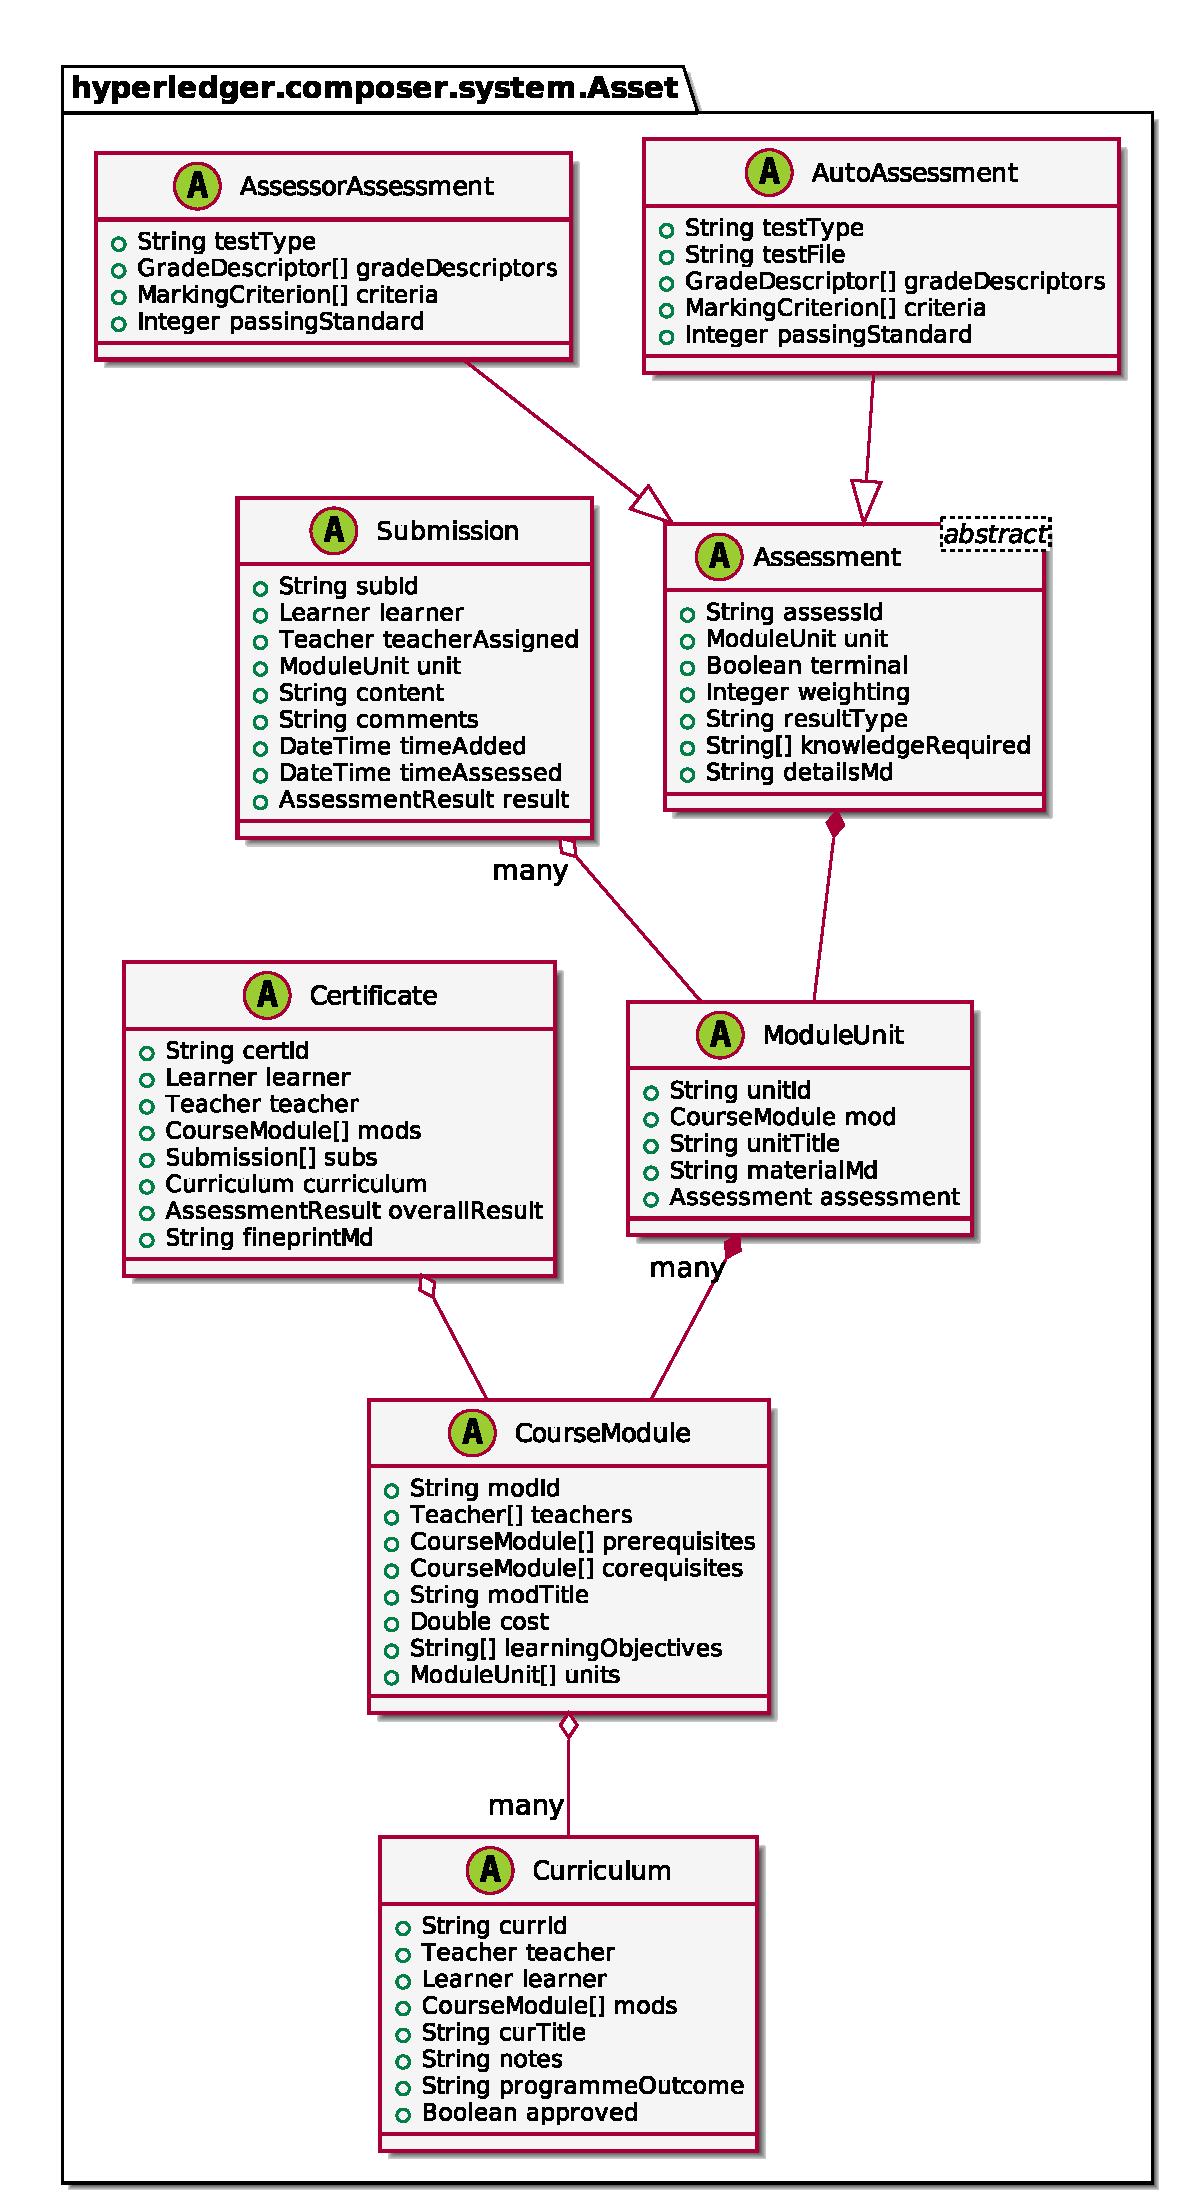
\includegraphics[width=0.6\textwidth]{assets}
    \caption[Assets Class Diagram]
        {Class diagram describing the assets defined on the blockchain} 
    \label{fig:assets}
\end{figure}

\begin{figure}[!ht] 
    \centering    
    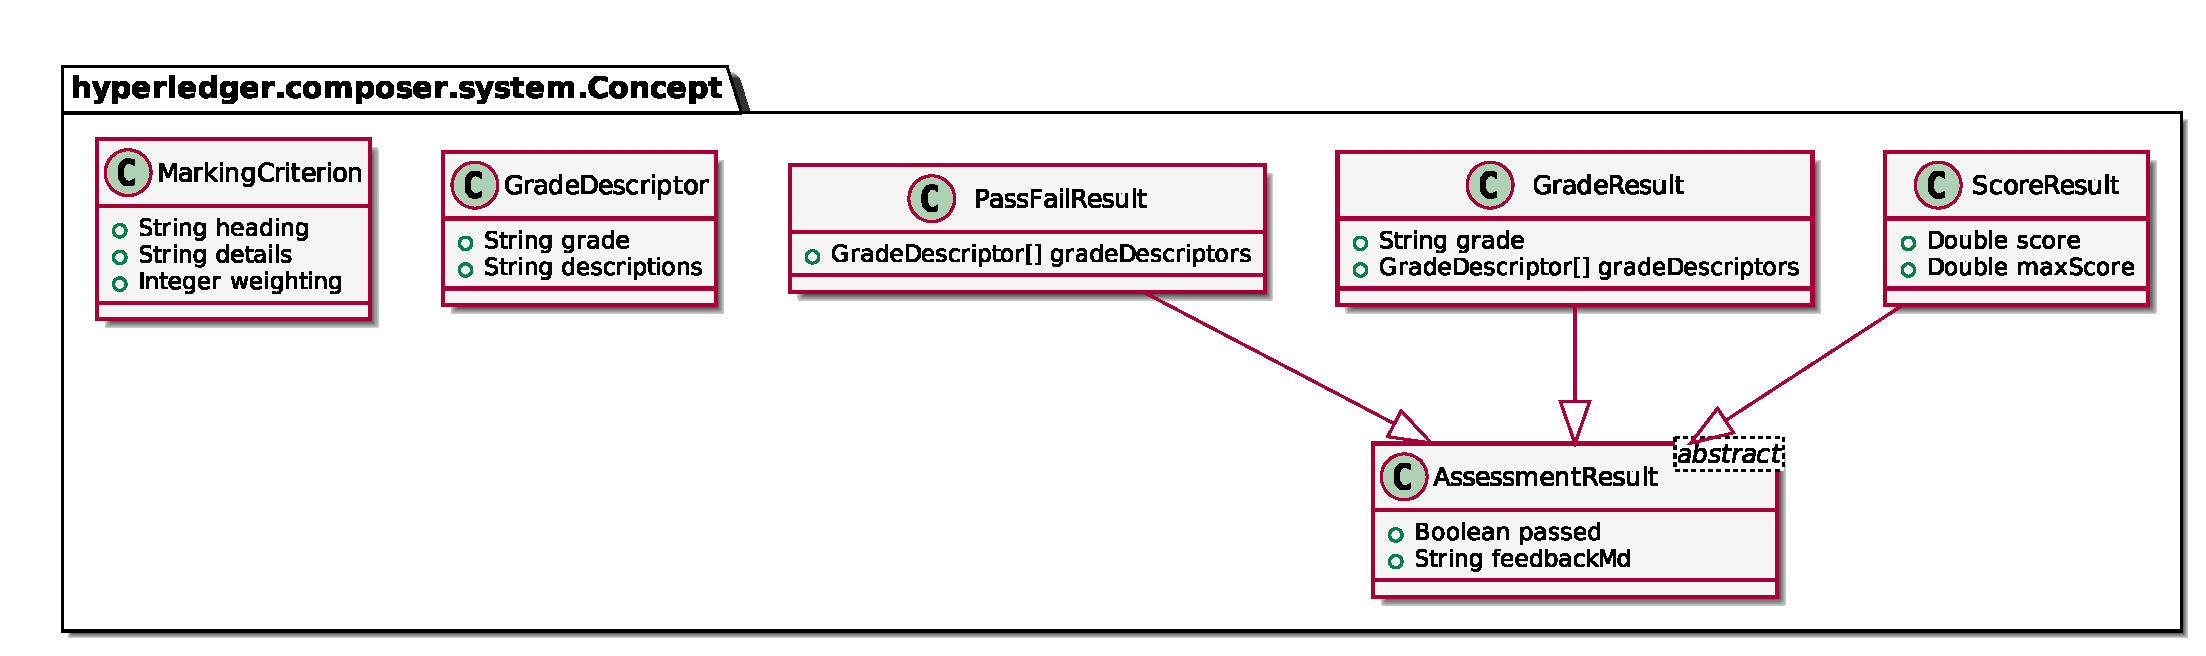
\includegraphics[width=1.0\textwidth]{concepts}
    \caption[Concepts Class Diagram]
        {Class diagram describing the concepts (other abstract classes that are contained as a field) defined on the blockchain} 
    \label{fig:concepts}
\end{figure}

\section{Smart Contracts: Transaction Logic and Events}
\begin{figure}[!ht]
    \centering
\begin{tikzpicture}[>=stealth,every node/.style={shape=rectangle,draw,rounded corners},]
    % create the nodes
    \node (start)[shape=circle, fill=gray, label=below:Tx Ordered] {};
    \node (c1) [right =of start, text width=1.5cm, align=center]{Integrity checks};
    \node (c2) [right =of c1, text width=4cm, align=center]{Adding new CourseModule, ModuleUnit, Assessment objects to blockchain};
    \node (c3) [right =of c2, text width=4cm, align=center]{Adding newly created CourseModule to the list of modules for each teacher};
    \node (stop1)[below =of c1, shape=circle, fill=gray, label=below:Tx Rejected] {};        
    \node (stop2)[right = of c3, shape=circle, fill=gray, label=below:Tx Accepted] {};    
    % connect the nodes
    \draw[->] (start) to (c1);
    \draw[->] (c1) -- node[anchor=south] {passed} (c2);
    \draw[->] (c1) -- node[anchor=west] {failed} (stop1);    
    \draw[->] (c2) to (c3);
    \draw[->] (c3) to (stop2);    
    % \draw[->] (c1.south) to[out=180,in=180] (c0.south);
\end{tikzpicture}
\caption{Smart Contract Logic for the Create Module Transaction (Tx)} \label{fig:cmtx}
\end{figure}
\section{Access Control}
Role based and attribute based

\section{Limitations}
No institutional approvers for certificates
No different tiers of privileges for teachers for roles such as module leader, module reviewer, supporting staff

\section{User Interfaces for Client Applications}
